% !TEX root = ../intro-stellar-physics.tex

\newcommand*{\altnuc}[3]{\ensuremath{\mathrm{_{#1}^{#2}#3}}}
\newcommand*{\nucarule}{\mbox{\rule[-5pt]{3.0em}{0.5pt}}}

To recap, we have established a description for the basic features of a self-gravitating fluid:
\begin{enumerate}

\item For a set mass and radius, hydrostatic equilibrium (balance of pressure and gravity) is established on the time needed for a sound wave to cross the star. Once this equilibrium is established, the central pressure, density, and temperature are established.

\item The gradient in temperature from center to surface drives a luminosity, which is controlled by the opacity of material in the stellar interior.

\item The ambient pressure and temperature near the stellar photosphere (where $\tau \sim 1$) are set by the surface gravity and opacity.

\end{enumerate}

In this chapter we now discuss how the luminosity is generated by nuclear reactions in the core of a star, and the conditions needed to generate that luminosity.

\section{The nucleus}

Experimentally, nuclei are on the order of femtometers\sidenote{$\val{1}{\fermi} = \val{10^{-15}}{\meter}$. This unit is sometimes called a \newterm{Fermi}.} in size. Like an atom, the nucleus also has excited states; typical energies for these states\sidenote{$\val{1}{\MeV} = \val{10^{6}}{\eV}$; an \newterm{electron volt} (eV) is the energy acquired by an electron being accelerated through a potential difference of 1 volt.} are on the order of MeV. It therefore makes sense to use fm and MeV as our units of length and energy. In these units, the combination
\[	\hbar c = \val{197}{\MeV\,\fermi} \]
to three significant digits. In quantum field theory, the strength of the electromagnetic interaction is characterized by the dimensionless \newterm{fine structure constant}
\[	\alphaF = \frac{e^{2}}{4\pi\epsilon_{0}\hbar c} = \frac{1}{137}, \]
again to three significant digits. From these two quantities, we find the electron (or proton) charge in these units,
\[
	\frac{e^{2}}{4\pi\epsilon_{0}} = \alphaF\hbar c = \val{1.44}{\MeV\,\fermi}.
\]
Put another way, the Coulomb potential energy between two protons separated by $\val{1}{\fermi}$ is $\val{1.44}{\MeV}$.

The strong nuclear force differs from electromagnetism and gravity in several ways. First, the strong nuclear force is short-range: the interaction vanishes for distances $\gtrsim\val{2}{\fermi}$. It is weakly attractive for distances $\val{1}{\fermi}\lesssim r\lesssim\val{2}{\fermi}$ and becomes strongly repulsive at distances $\ll\val{1}{\fermi}$. The potential between the neutron and proton in a deuterium (\hydrogen[2]) nucleus (called a deuteron) therefore looks something like that sketched in Fig.~\ref{f.nuclear-potential}. The deuteron's ground state (black dotted line) is at $E_{\mathrm{d}} = -\val{2.2}{\MeV}$, so the nucleus is weakly bound ($|E_{\mathrm{d}}| \ll |V|$, where $V$ is the depth of the potential well).

\begin{marginfigure}[-8\baselineskip]
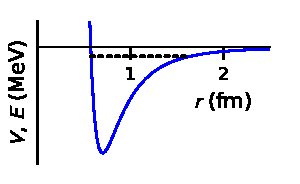
\includegraphics[width=\linewidth]{nuclear-potential}
\caption[Schematic of the nuclear potential]{\label{f.nuclear-potential}Schematic of the nuclear potential for a deuteron (\hydrogen[2]). The binding energy of the deuteron is shown as a black dotted line.}
\end{marginfigure}

\marginnote{In our units of MeV and fm, some relevant masses are
\begin{eqnarray*}
m_{n} &=& \val{939.6}{\MeV}/c^{2}\\
m_{p} &=& \val{938.3}{\MeV}/c^{2}\\
\mb &=& \val{931.5}{\MeV}/c^{2}\\
m_{e} &=& \val{0.5110}{\MeV}/c^{2}
\end{eqnarray*}
}

\begin{exercisebox}[Depth of nuclear well]
We can estimate the depth of the well in Fig.~\ref{f.nuclear-potential}. Since this is a two-body problem, transfer to center-of-mass coordinates and solve for a single particle with a reduced mass $m_{p}m_{n}/(m_{p}+m_{n}) \approx m_{n}/2$. Use the uncertainty principle, with $\Delta x$ being the width of the well, to get an estimate of $p\sim\Delta p$ and from this estimate the kinetic energy of the particle. Finally, use the small value of the binding energy (sum of potential and kinetic energies) to estimate the depth of the potential well.
\end{exercisebox}

Also unlike electromagnetism and gravity, the strong nuclear force does not obey superposition: we cannot write the energy of the nucleus as a sum over the potential between all pairs of nucleons. Further, the strong nuclear force is not a central force, meaning that it depends on more than just the distance between any two nucleons. The atomic nucleus is thus much more complicated to describe than the electronic structure of the atom.

\newthought{Despite these complications, we can construct a phenomenological formula for the nuclear mass that is reasonably accurate.} Let us write the mass of a nucleus with $A$ nucleons---$Z$ protons and $N=A-Z$ neutrons---as
\[
	M(Z,N) = Zm_{p} + Nm_{n} - B(Z,N)/c^{2},
\]
where $B(Z,N)$ is the \newterm{binding energy}---the amount of energy that must be supplied to the nucleus in order to break it into its constituent protons and neutrons.
Because the nuclear force is weakly attractive for separations $\val{1}{\fermi}\lesssim r\lesssim\val{2}{\fermi}$ and repulsive at shorter distances (Fig.~\ref{f.nuclear-potential}), there is a characteristic spacing between nucleons that is a bit larger than $\val{1}{\fermi}$. In a large nucleus, we therefore expect the nucleons to have a roughly constant density, so that the volume of the nucleus is proportional to $A$; experimentally, the radius of the nucleus is roughly\sidenote{The value of the radius depends on how it is measured; scattering with various light particles (protons, neutrons, alpha, electrons) agree, however, that $r_{A}\propto A^{1/3}$.}
\[
	r_{A} = \valrng{1.1}{1.8}{\fermi}\times A^{1/3}.
\]
Notice that because the nucleon-nucleon potential is short-ranged, nucleons in a large nucleus only interact with their nearest neighbors. Indeed the nucleon-nucleon interaction is similar in form to the potential between molecules in a fluid, such as a water drop. This motivates developing a simple formula that gives a decent approximation for the binding energy. For the first term, we estimate the binding energy of a large nucleus as just the (constant) binding energy of a single nucleon multiplied by the number of nucleons. Experimentally, it is found that for large nuclei this is the case: the binding energy per nucleon is roughly constant. We say that the nuclear interaction \newterm{saturates}, so that $B(Z,N) \propto A = (Z+N)$.

\begin{exercisebox}[If the strong force were long-range]
To see how the nuclear force differs from the long-range Coulomb and gravitational forces, suppose instead that the nuclear force acted like a super-gravity: that is, the potential was $\propto 1/r$. Use the results from our constant-density model of a star (eq.~[\ref{e.energy-constant-density-sphere}]) to derive how the binding energy would scale with $A$ in this case.
\end{exercisebox}

It is energetically favorable to have equal numbers of neutrons and protons. We therefore define an asymmetry parameter $\eta \equiv (N-Z)/(N+Z) = 1-2Z/A$, so that $-1\le\eta\le1$. The nuclear contribution to the binding energy is maximized for $\eta = 0$ (equal numbers of protons and neutrons). Because the nuclear force does not distinguish between neutrons and protons, the binding energy is quadratic in $\eta$, so that $B$ doesn't depend on the sign of $\eta$. Thus our first approximation for the binding energy is $B \approx (a_{V} - a_{A}\eta^{2}) A$. Here $a_{V}$ and $a_{A}$ are as-yet-undetermined coefficients.

In a fluid drop there is a correction for the surface tension. Heuristically, we imagine that nuclei in the surface have fewer neighbors and are therefore not as bound. We therefore subtract from our formula a term proportional to the surface area, $\propto r_{A}^{2} \propto A^{2/3}$. The next iteration of our liquid-drop approximation is thus $B \approx (a_{V}- a_{A}\eta^{2})A - a_{S}A^{2/3} $.

Finally, the protons in the nucleus are charged and therefore repel one another. This Coulomb repulsion also reduces the binding energy. We therefore subtract a term $\propto Z^{2}/r_{A}\propto Z^{2}/A^{1/3}$ from our mass formula to obtain
\begin{equation}\label{e.liquid-drop}
B = \left(a_{V} -a_{A}\eta^{2}\right) A -  a_{S}A^{2/3} - a_{C} \frac{Z^{2}}{A^{1/3}}. 
\end{equation}
This is a version of the \newterm{semi-empirical mass formula}, also known as the \newterm{Bethe-Weizs\"acker mass formula}.
The coefficients $a_{V},a_{A},a_{S},a_{C}$ are found by fitting the formula to measured nuclear masses (Table~\ref{t.liquid-drop}).
\begin{margintable}
\caption[Liquid-drop coefficients]{\label{t.liquid-drop} Coefficients for the fit to nuclear masses, (\protect\ref{e.liquid-drop}), in units of MeV.}
\begin{tabular}{rrrr}
$a_V$ & $a_A$ & $a_S$ & $a_C$ \\
\hline
15.5 & 22.7 & 16.6 & 0.71\\
\end{tabular}
\end{margintable}
\noindent This fit should have another term to account for the pairing of neutrons and protons, so that the binding energy is increased for even $Z$ and $N$. We omit that term here for simplicity.

\begin{exercisebox}[The nuclear landscape \notebook]
\label{ex.nuclear-landscape}
\notebook~For a given nuclear mass number $A$, derive an expression for the charge number $Z_{\star}(A)$ that maximizes the binding energy (eq.~[\ref{e.liquid-drop}] with coefficients from Table~\ref{t.liquid-drop}).
\begin{enumerate}
\item Plot the ratio $Z_{\star}/A$ for $4\le A\le 128$. Give a physical explanation for the behavior of $Z_{\star}/A$.
\item Plot the binding energy per nucleon $B/A$ as a function of $Z_{\star}$ and $A$, for $4\le A\le 128$.
\item Find the atomic number $Z$ and atomic mass $A$ of the nucleus with the maximum $B/A$.
\end{enumerate}
\end{exercisebox}

\section{Nuclear reactions}

From mass-energy conservation, the heat evolved during a nuclear reaction equals the change in mass of the reacting system. For example, in the reaction
\[
	\helium[3] + \helium[3] \to \helium + \pt + \pt,
\]
the binding energy of \helium[3] is \val{7.718}{\MeV} and that of \helium\ is \val{28.296}{\MeV}; the heat evolved by this reaction is therefore
\begin{eqnarray*}
	\lefteqn{2\left[2m_{p}+m_{n}-B(\helium[3])\right] - \left[2m_{p}+2m_{n}-B(\helium)\right] - 2m_{p}} \\
	&=& B(\helium)-2B(\helium[3])\\
	&=& \val{28.296}{\MeV} - \val{15.437}{\MeV}\\ &=& \val{12.859}{\MeV}.
\end{eqnarray*}
\begin{exercisebox}[Heat from hydrogen fusing to helium]
\label{ex.Q-hydrogen-helium}
Fusion of hydrogen into helium entails converting 4 hydrogen atoms (including the 4 electrons) into 1 helium atom (2 protons, 2 neutrons, 2 electrons) with $B = \val{28.296}{\MeV}$. What is the heat evolved \emph{per hydrogen atom}? Assume that the sun has been shining with its current luminosity over its life. What mass of hydrogen atoms would need to undergo fusion to supply this energy? How large is this mass relative to the total mass of the sun? 
\end{exercisebox}

\begin{margintable}
\caption[Selected atomic mass excesses]{\label{t.atomic-mass-excesses} Selected atomic mass excesses, taken from \protect\citet{Tuli2011Nuclear-Wallet-}.}
\begin{tabular}{ld{7.3}}
\tabhead{isotope} & \tabhead{$\Delta/\MeV$}\\
\hline
\nt & 8.071 \\
\hydrogen & 7.289 \\
\helium &   2.425 \\
\carbon &   0.000 \\
\oxygen &  -4.737 \\
\silicon& -21.493 \\
\iron   & -60.606 \\
\end{tabular}
\end{margintable}Because stellar reactions often involve electrons, it is convenient to define the \newterm{atomic mass excess} $\Delta(Z,A) = \mathcal{M}(Z,A) - A\mb$, where $\mathcal{M}$ is the atomic mass, including electrons.\marginnote{From the definition of the atomic mass unit $\mb$, 
$\Delta(\carbon) \equiv 0$.}
Some common mass excesses are listed in Table~\ref{t.atomic-mass-excesses}.
Neglecting the electron binding energy ($\sim\eV$), we can relate the atomic mass excess to the binding energy via $\mathcal{M}(Z,A) = A\mb + \Delta(Z,A) = M(Z,N=A-Z) + Z m_{e}$.

\begin{exercisebox}[Energy released by various reactions]
\label{ex.energy-release}
Compute the energy released by the following reactions:
\begin{eqnarray*}
\helium+\helium+\helium &\to& \carbon\\
\carbon + \helium &\to& \oxygen\\
\oxygen + \oxygen &\to& \silicon + \helium.
\end{eqnarray*}
\end{exercisebox}

\newthought{You might think that because the nuclear interaction is short-range, the cross-section is something like $\pi r_{n}^{2}$, where $r_{n}\approx\valrng{1}{2}{\fermi}\times A^{1/3}$.} Things are a bit more subtle, however, and in this section we shall explore how the reaction rate works. First, the ``size'' of a particle is in general proportional to the ``size'' of the wavefunction. From the uncertainty principle, 
\[\pi\,\Delta x^{2} \approx \pi \left(\frac{\hbar}{\Delta p}\right)^{2} = \pi\frac{\hbar^{2}}{2mE}.\]
where we've taken $\Delta p\sim p$.
Notice that if we multiply and divide by $c^{2}$, then we can estimate the area of the wavepacket as
\[
	\frac{(\hbar c)^{2}}{m_{p} c^{2}} \frac{1}{E} \sim \val{\sci{4}{4}}{\fermi^{2}} \times \left(\frac{\keV}{E}\right) = \val{400}{\barn}\left(\frac{\keV}{E}\right).
\]	
Here we've introduced a convenient unit for nuclear cross-sections, the \newterm{barn}\sidenote{as in hitting the broad side of} (b), with $\val{1}{\barn} = \val{10^{-28}}{\meter^{2}} = \val{100}{\fermi^{2}}$.

The key point is that the size of the wave packet is $\propto 1/E$, which is in general true. This geometrical size of the wave packet is then multiplied by the probability of the nucleons forming a bound state, so we write the nuclear portion of the cross-section as
\begin{equation}\label{e.nuclear-cross-section}
	\sigma_{\mathrm{nuclear}}(E) = \frac{S(E)}{E}.
\end{equation}
The function $S(E)$ contains the details of the nuclear interaction and is in general measured experimentally.

The final part of the cross-section concerns the Coulomb potential.
Because protons repel one another, at large separations the nuclei interact \emph{only} via the Coulomb potential. Consider the case of two nuclei with masses\sidenote{When doing kinematics, we shall make the approximation $m\approx A\mb$.} $A_{1}\mb$ and $A_{2}\mb$. Transform to the center-of-mass frame; the problem then reduces to that of one particle, mass $A\mb = A_{1}A_{2}/(A_{1}+A_{2})\times\mb$, moving in a potential (Fig.~\ref{f.tunneling}) that at large separations is purely Coulomb,
\[ \frac{Z_{1}Z_{2}e^{2}}{4\pi\epsilon_{0}r} = \frac{Z_{1}Z_{2}\alphaF\hbar c}{r} = \val{1.44}{\MeV}\times Z_{1}Z_{2}\left(\frac{\val{1}{\fermi}}{r}\right). \]
Although the nuclear interaction forms a deep potential well (blue $V_{n}$, Fig.~\ref{f.tunneling}) at short distances, outside the nucleus the Coulomb potential (red $V_{C}$, Fig.~\ref{f.tunneling})  dominates.
\begin{marginfigure}[-8\baselineskip]
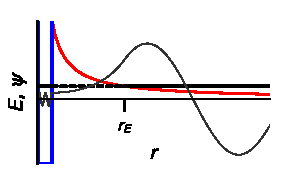
\includegraphics[width=\linewidth]{tunnel-schematic}
\caption[Tunneling through the Coulomb potential barrier]{Tunneling through the Coulomb potential barrier. Not to scale.}
\label{f.tunneling}
\end{marginfigure}

\begin{exercisebox}[Turning radius for proton-proton collision in solar plasma]
\label{ex.turning-radius}
For the sun, typical center-of-mass energies are $E \sim \val{1}{\keV}$ (horizontal black line in Fig.~\ref{f.tunneling}). Suppose we have two protons heading towards one another with this kinetic  energy. What is their distance of closest approach?
\end{exercisebox}

As shown in Exercise~\ref{ex.turning-radius}, the turning radius $r_{E}$ at typical stellar energies is much larger than the nuclear radius.  Classically the particle can't penetrate the region $r_{n} < r < r_{E}$ where $E < V$ (dotted black line, Fig.~\ref{f.tunneling}); under classical physics, there would be no nuclear reactions at typical stellar temperatures because two particles would never find themselves close enough to be bound by the nuclear force.

The world is quantum, however, and the uncertainty in a particle's position means there is a small probability for the nucleons to be close enough for the nuclear force to come into play. In the classically forbidden region $r_{n} < r < r_{E}$, the particle wavefunction (thin gray line, Fig.~\ref{f.tunneling}) decreases exponentially, and the probability to reach $r\sim\val{1}{\fermi}$ is
\[ \mathcal{P}\approx \exp\left[-2\pi^{2}\frac{r_{E}}{\lambda}\right] \]
where $\lambda = h/p$ is the particle's wavelength and $p$ is the momentum.
It is convenient to rewrite the argument of the exponential in terms of the particle's energy,
\[ \frac{2\pi^{2}r_{E}}{\lambda} = 2\pi^{2}\left(\frac{Z_{1}Z_{2}e^{2}}{E}\right)
	\left(\frac{p}{h}\right) = \left[\pi \frac{Z_{1}Z_{2}e^{2}\sqrt{2m}}{\hbar}\right]\left(\frac{1}{E}\right)^{1/2}, \]
so that the probability of ``tunneling'' through the Coulomb barrier is
\begin{equation}\label{e.probability-tunneling}
\mathcal{P} \approx \exp\left[-\left(\frac{\EG}{E}\right)^{1/2}\right],
\end{equation}
with
\[ \EG \equiv \textrm{``Gamow Energy''} = \left[\frac{2\pi^{2}Z_{1}^{2}Z_{2}^{2}e^{4}m}{\hbar^{2}}\right] = Z_{1}^{2}Z_{2}^{2}A \times \val{979}{\keV}.
\]
Combining eqs.~(\ref{e.nuclear-cross-section}) and (\ref{e.probability-tunneling}), we write the reaction cross-section as the nuclear cross-section multiplied by the probability of tunneling:
\begin{equation}\label{e.s-def}
\sigma(E) = \frac{S(E)}{E}\exp\left[-\left(\frac{\EG}{E}\right)^{1/2}\right].
\end{equation}
For many reactions $S(E)$ is nearly constant over the range of typical energies in a stellar plasma. This is useful, as the reaction cross-section can be measured in the lab at higher energies and then extrapolated to the much lower stellar energies using eq.~(\ref{e.s-def}).

\newthought{To get the reaction rate from the cross-section,} recall that the mean-free path of a particle is $\ell = (n\sigma)^{-1}$, where $n$ is the density of targets. For definiteness, let us consider a plasma with two species present, type 1 and type 2. The mean-free path of any given nucleus of type 1 against reactions with nuclei of type 2 is $\ell = (n_{2}\sigma)^{-1}$. If the nuclei are traveling with relative speed $v = |\bvec{v}_{1}-\bvec{v}_{2}|$, then the mean time between collisions is $\ell/v$. Thus in a large ensemble of nuclei, the mean rate of reactions is
\begin{equation}\label{e.mean-reaction-rate}
	r_{12} = \frac{n_{1} v}{\ell} = n_{2}n_{1}\langle\sigma v\rangle.
\end{equation}
Here $\langle \sigma v\rangle$ is the mean value of $\sigma v$ for all pairs of nuclei in the plasma. For reactions between nuclei of the same type, we replace $n_{1}n_{2}$ with $n^{2}/2$; the factor of $1/2$ is to avoid double-counting.

A detailed calculation of the thermally averaged cross-section $\langle\sigma v\rangle$ is presented in Box~\ref{sb.thermally-averaged-cross-section}; here we'll just give a brief physical explanation for its value. There are two competing terms. First, the cross-section (eq.~\ref{e.s-def}) has an exponential term $\exp[-(\EG/E)^{1/2}]$ that increases rapidly with energy: more energetic particles have a much higher probability of tunneling through the Coulomb barrier. On the other hand, in thermal equilibrium the number of particles with energy $E$ decreases as $\exp(-E/\kB T)$.
As a result, reactions predominately occur in a narrow window of energies about a sort of geometric mean between \EG\ and $\kB T$:
\[	\Epk = \frac{\EG^{1/3}(\kB T)^{2/3}}{4^{1/3}}. \]
The reaction rate is suppressed for $E\ll\Epk$ because the probability of penetrating the Coulomb barrier is so small; the reaction rate is suppressed for $E\gg\Epk$ because there are so few nuclei with those energies. Using this approximation the rate can be evaluated, with $\langle\sigma v\rangle$ being given by eq.~(\ref{e.rate2}).

\begin{sidebar}[The thermally averaged reaction cross-section]
\label{sb.thermally-averaged-cross-section}
Since the cross-section depends on energy, the rate at which any given nucleus of type 1, traveling with velocity $\bvec{v}_{1}$, will react with nuclei of type 2 having velocities $\bvec{v}_{2}$ in a range $\dif^{3}v_{2}$ is
\[ n_{2} \sigma |\bvec{v}_{1}-\bvec{v}_{2}| \left(\frac{m_{2}}{2\pi \kB T}\right)^{3/2}\exp\left(-\frac{m_{2}v_{2}^{2}}{2\kB T}\right) \,\dif^{3}v_{2}. \]
The extra terms are because the nuclei have a Maxwell-Boltzmann distribution of velocities. To get the total rate per unit volume, we then have to multiply by the number of nuclei of type 1 having velocities $\bvec{v}_{1}$ in a range $\dif^{3} v_{1}$ and integrate over $\dif^{3}v_{1}\,\dif^{3}v_{2}$:
\begin{eqnarray}\label{e.rate-joint}
\lefteqn{r_{12} = n_{1}n_{2}  \left[\frac{m_{1}m_{2}}{(2\pi \kB T)^{2}}\right]^{3/2}}
  \nonumber\\ &&\times\int\! \sigma(E) v\exp\left(-\frac{m_{1}v_{1}^{2}}{2\kB T}-\frac{m_{2}v_{2}^{2}}{2\kB T}\right)  \,\dif^{3} v_{1}\,\dif^{3}v_{2}.
\end{eqnarray}
Now $E$ and $v$ are the relative energies and velocity in the center-of-mass frame.  We can change variable using the relations
\begin{eqnarray*}
\bvec{v}_{1} &=& \bvec{V} - \frac{m_{2}}{m_{1}+m_{2}} \bvec{v}\\
\bvec{v}_{2} &=& \bvec{V} + \frac{m_{1}}{m_{1}+m_{2}} \bvec{v}.
\end{eqnarray*}
where $V$ is the center-of-mass velocity. It is straightforward to show that $\dif v_{1,x}\,\dif v_{2,x} = \dif V_{x}\dif v_{x}$, and likewise for the $y,z$ directions.  Furthermore, $m_{1}v_{1}^{2} + m_{2}v_{2}^{2} = (m_{1}+m_{2})V^{2} + m v^{2}$, and multiplying and dividing the integral in equation~(\ref{e.rate-joint}) by $m_{1}+m_{2}$ allows us to write
\begin{eqnarray*}
\lefteqn{r_{12} = n_{1}n_{2} \left(\frac{m_{1}+m_{2}}{2\kB T}\right)^{3/2}\left(\frac{m}{2\kB T}\right)^{3/2}}\\
&&\times \int\!\dif^{3}V \int\!\dif^{3}v \,\sigma(E)v \exp\left[-\frac{mv^{2}}{2\kB T}\right]
 \exp\left[-\frac{(m_{1}+m_{2})V^{2}}{2\kB T}\right].
\end{eqnarray*}
The integral over $\dif^{3}V$ can be factored out and is normalized to unity. Hence we have for the reaction rate between a pair of nuclei of types 1 and 2, 
\begin{eqnarray}\label{e.rate}
r_{12} &=& n_{1}n_{2}\left\{\left(\frac{m}{2\pi\kB T}\right)^{3/2}\int_{0}^{\infty}\! \sigma(E) v \exp\left(-\frac{mv^{2}}{2\kB T}\right)  4\pi v^{2}\,\dif v\right\}.\nonumber\\
 &\equiv& n_{1}n_{2}\langle\sigma v\rangle.
\end{eqnarray}
The term in $\{\}$ is the averaging over the joint distribution of the cross-section times the velocity, and is usually denoted as $\langle\sigma v\rangle$. Note that if nuclei 1 and 2 were identical, then we would need to divide $r_{12}$ by 2.

Changing variables to $E = mv^{2}/2$ in equation~(\ref{e.rate}) and inserting the formula for the cross-section, equation~(\ref{e.s-def}), gives
\begin{equation}\label{e.integral}
\langle\sigma v\rangle = \left(\frac{8}{\pi m}\right)^{1/2}\left(\frac{1}{\kB T}\right)^{3/2}\int_{0}^{\infty}\!S(E)\exp\left[-\left(\frac{\EG}{E}\right)^{1/2}-\frac{E}{\kB T}\right]\,\dif E.
\end{equation}
Now, we've assumed that $S(E)$ varies slowly; but look at the argument of the exponential. This is a competition between a rapidly rising term $\exp[-(\EG/E)^{1/2}]$ and a rapidly falling term $\exp(-E/\kB T)$. As a result, the exponential will have a strong peak, and we can expand the integrand in a Taylor series about the maximum. Let 
\[
f(E) = -\left(\frac{\EG}{E}\right)^{1/2} - \frac{E}{\kB T}.
\]
Then we can write 
\begin{eqnarray*}
\lefteqn{\int_{0}^{\infty}\!S(E)\exp\left[-\left(\frac{\EG}{E}\right)^{1/2}-\frac{E}{\kB T}\right]\,\dif E}\\
&\approx&
	\int_{0}^{\infty}\! S(\Epk)\exp\left[f(\Epk) + \frac{1}{2}\left.\frac{\dif^{2} f}{\dif E^{2}}\right|_{E=\Epk}\left(E-\Epk\right)^{2}\right]\,\dif E.
\end{eqnarray*}
Here $\Epk$ is found by solving $(\dif f/\dif E)|_{E=\Epk} = 0$. By expanding the argument of the exponential, we have approximated the integrand by a Gaussian,
\[
	\exp\left[-\frac{(E-\Epk)^{2}}{2\varsigma^{2}}\right]
\]
where
\[
	\frac{1}{\varsigma^{2}} = -\left.\frac{\dif^{2} f}{\dif E^{2}}\right|_{E=\Epk}.
\]
This trick of approximating a steeply peaked function as a Gaussian is known as the \newterm{method of steepest descent}.

Solving for \Epk, we get
\[
\Epk = \frac{\EG^{1/3}(\kB T)^{2/3}}{2^{2/3}},
\]
and 
\[ \exp\left[f(\Epk)\right] = \exp\left[-3\left(\frac{\EG}{4\kB T}\right)^{1/3}\right].
\]
Further,
\[
\left.\frac{1}{2}\frac{\dif^{2}f}{\dif E^{2}}\right|_{E=\Epk} = -\frac{3}{2(2\EG)^{1/3}(\kB T)^{5/3}} = -\frac{3}{4\Epk \kB T}.
\]
Defining a variable $\Delta = 4(\Epk \kB T/3)^{1/2}$, our integral becomes
\begin{eqnarray}\label{e.integral2}
\lefteqn{\langle\sigma v\rangle = \left(\frac{8}{\pi m}\right)^{1/2}\left(\frac{1}{\kB T}\right)^{3/2} S(\Epk)} \nonumber\\
&&\times 
  \exp\left[-3\left(\frac{\EG}{4\kB T}\right)^{1/3}\right]\int_{0}^{\infty}\!\exp\left[-\frac{(E-\Epk)^{2}}{(\Delta/2)^{2}}\right]\,\dif E.
\end{eqnarray}
Another simplification can be made because both the Gaussian and the original integrand go to zero as $E\to 0$.  As a result, we can extend the lower bound of our integral (eq.~[\ref{e.integral2}]) to $-\infty$, which allows us to evaluate the integral analytically and obtain
\begin{eqnarray}\label{e.rate2}
\langle\sigma v\rangle &\approx& \left(\frac{8}{m}\right)^{1/2}\left(\frac{1}{\kB T}\right)^{3/2} S(\Epk) \exp\left[-3\left(\frac{\EG}{4\kB T}\right)^{1/3}\right] \frac{\Delta}{2}\nonumber\\
 &=& \frac{2^{13/6}}{\sqrt{3m}}\frac{\EG^{1/6}S(\Epk)}{(\kB T)^{2/3}} \exp\left[-3\left(\frac{\EG}{4\kB T}\right)^{1/3}\right]  .
\end{eqnarray}
\end{sidebar}

The rate has the temperature dependence
\[
	r \propto T^{-2/3} \exp\left[-3\left(\frac{\EG}{4\kB T}\right)^{1/3}\right];
\]
since $\EG \propto Z_{1}^{2}Z_{2}^{2}A$, at any given temperature lighter nuclei typically have much faster reaction rates. Also note that at stellar energies, reaction rates are incredibly sensitive to temperature. To quantify this, approximate the rate at a given temperature as a power-law, $r(T)\propto T^{n}$. Then the exponent is
\begin{equation}\label{e.exponent}
 n(T) = \dd{\ln r}{\ln T} = -\frac{2}{3} + \left(\frac{\EG}{4\kB T}\right)^{1/3},
\end{equation}
as you can verify for yourself (Exercise~\ref{ex.power-law}). Table~\ref{t.reaction} lists $\EG$, $\Epk$, and $n$ for some common reactions. 
In the table, the peak reaction energy $\Epk$ and exponent $n(T)$ are evaluated at $T = \val{10^{7}}{\K}$ ($\kB T = \val{0.86}{\keV}$). Note the large value of $n(T)$ at stellar temperatures---this is a consequence of the largeness of $\EG/\kB T$.
 
\begin{table}[hb]
\caption{\label{t.reaction} Parameters for non-resonant reactions}
\begin{tabular}{lrrrrrr}
 & $\pt+\pt$ & $\pt+\helium[3]$ & $\helium[3]+\helium[3]$ & $\pt+\lithium[7]$ & $\pt+\carbon$\\
\hline
%$A$ & 1/2 & 3/4 & 3/2 & 0.88 & 0.92 \\
%$Z_{1}Z_{2}$ & 1 & 2 & 4 & 3 & 6 \\
$\EG$ (MeV) & 0.489 & $2.94$ & $23.5$ & $7.70$ & $32.5$\\
%$\EG/(4k)$ (GK) & $1.4$ & $8.5$ & $68.0$ & $22.0$ & $94.0$ \\
$\Epk|_{T=\val{10^{7}}{\K}}$ (keV) & 4.5 & 8.2 & 16.3 & 11.3 & 18.2\\
%$\Delta/\Epk|_{T=\val{10^{7}}{\K}}$ & 1.0 & 0.75 & 0.53 & 0.64 & 0.50 \\
$n(T = \val{10^{7}}{\K})$ & 4.6 & 8.8 & 18.3 & 12.4 & 20.5\\
\end{tabular}
\end{table}

\begin{exercisebox}[Approximating a function as a power-law]
\label{ex.power-law}
Suppose we wish to approximate a function $f(x)$ at a point $x_{0}$ with a power-law, $p(x;A,n) = Ax^{n}$. Impose the condition $p(x_{0};A,n) = f(x_{0})$ and $\dif p/\dif x |_{x=x_{0}} = \dif f/\dif x|_{x=x_{0}}$ to find the parameters $A$ and $n$, and show that
\[
	n = \DD{\ln f}{\ln x}.
\]
Apply this to the reaction rate, eq.~(\ref{e.rate2}), and thus derive eq.~(\ref{e.exponent}).
\end{exercisebox}

\section{Stellar nuclear reactions}

\subsection{Hydrogen burning via pp reactions: the weak nuclear interaction}

In the previous section, we established that lighter nuclei, because of their lower Coulomb repulsion, will tend to fuse at lower temperatures. Thus we expect that the first reaction that can occur is $\pt+\pt$ and therein lies a problem: there is no bound state of \helium[2]. The only possible way for two protons to fuse is for one of the protons to transmute into a neutron, giving the reaction
\begin{equation}\label{e.pp}
	\pt + \pt \to \hydrogen[2] + e^{+} + \nu_{e}.
\end{equation}
This reaction is possible because there are two nuclear forces: the strong and the weak. The strong is what binds nuclei together\marginnote{More precisely, what the strong force mainly does is bind quarks into neutrons or protons.}; the weak mediates the conversion of a neutron into a proton (and vice versa). Two leptons are also involved (either emitted or absorbed) in this type of weak reaction: an electron (or its anti-particle, the positron) and an electron neutrino (or anti-neutrino). Three conservation laws determine which particles are involved:
\begin{enumerate}
\item\label{i.baryon-conservation} the number of nucleons is conserved;
\item\label{i.charge-conservation} the charge is conserved; and
\item\label{i.lepton-conservation} the number of leptons is conserved.
\end{enumerate}
With regard to item \ref{i.lepton-conservation}, electrons ($e^{-}$) and electron neutrinos ($\nu_{e}$) have lepton number $+1$ while positrons ($e^{+}$) and anti-electron neutrinos ($\bar{\nu}_{e}$) have lepton number $-1$. Neutrinos, as the name implies, do not carry charge.

Applying these rules to the reaction (\ref{e.pp}), the number of nucleons on both sides of this reaction is the same, so rule \ref{i.baryon-conservation} is satisfied. The positron on the right hand side balances charge to satisfy rule \ref{i.charge-conservation}. Finally, the emission of an electron neutrino ensures that the lepton number on the right-hand side is zero to satisfy rule \ref{i.lepton-conservation}.

\begin{exercisebox}[Conservation laws applied to reactions]
Complete the following reactions. Note that the symbol $_{Z}^{A}\mathrm{El}$ indicates that nuclide ``El'' has atomic charge number $Z$ and atomic mass number $A$.
\begin{eqnarray*}
\altnuc{27}{56}{Co} +  \nucarule &\to& \altnuc{26}{56}{Fe} + \nu_{e}\\
\altnuc{6}{13}{C} + \altnuc{2}{4}{He} &\to& \nt + \nucarule\\
\altnuc{6}{14}{C} &\to& \nucarule + \nucarule + \bar{\nu}_{e}\\
\altnuc{10}{21}{Na} + \altnuc{2}{4}{He} &\to& \pt + \nucarule\\
\end{eqnarray*}
\end{exercisebox}

The weak cross section goes roughly as $\sigma_{\mathrm{weak}} \sim \val{10^{-20}}{\barn}\left(E/\keV\right)$, so that
\[ \frac{\sigma_{\mathrm{weak}}}{\sigma_{\mathrm{nuc}}} \sim 10^{-23}\left(\frac{E}{\keV}\right). \]
As a result the characteristic temperature for reaction (\ref{e.pp}) to occur is $\approx \val{\sci{1.5}{7}}{\K}$, much higher than the temperature at which $\pt+\hydrogen[2]$ occurs; at this temperature, the lifetime of a proton to forming deuterium via capture of another proton is about $\val{6}{\Giga\yr}$.
\marginnote{Because the weak cross section is so small, the first reaction that occurs in a contracting pre-main sequence star is $\hydrogen[2]+\pt\to\helium[3]$; in fact, this reaction can occur in objects as small as $\approx \val{12}{M_{\mathrm{Jupiter}}}$. The small primordial abundance of deuterium prevents this reaction from doing anything more than slowing contraction slightly.}
Once a deuterium nucleus is formed, it is immediately destroyed via $\hydrogen[2]+\pt\to\helium[3]$. The reaction $\pt + \helium[3]\to\lithium[4]$ cannot occur because \lithium[4] is unbound and decays back into $\pt+\helium[3]$ with a lifetime of $\val{10^{-22}}{\second}$. 
The nucleus \beryllium[6] is likewise unbound ($\tau \sim \val{\sci{5}{-21}}{\second}$), but it decays into two $\pt$ and a $\helium[4]$ nucleus. As a result, the next reaction that occurs is $\helium[3]+\helium[3]\to \pt+\pt+\helium$. Despite having a much greater Gamow energy than $\pt + \pt$, this reaction is still much faster than $\pt+\pt$ owing to the small weak cross-section.

In addition to capturing another \helium[3], it is also possible for \helium[3] to react with \helium\ and trigger the reactions
\marginnote{In eq.~(\ref{e.pp-2}) and (\ref{e.pp-3}), $\tau$ refers to the half-life for the nucleus on the left.}
\begin{eqnarray}
\helium[3] + \helium &\to& \beryllium[7] + \gamma\nonumber\\
 \beryllium[7] + e^{-} &\to& \lithium[7] +  \nu_{e}\qquad(\tau=\val{53}{\unitstyle{d}})\nonumber \\
 \lithium[7] + \pt &\to& \helium+\helium + \gamma;
\label{e.pp-2}
\end{eqnarray}
furthermore, at slightly higher temperatures \beryllium[7] can capture a proton instead of an electron to yield
\begin{eqnarray}
\beryllium[7] + \pt &\to& \boron[8] + \gamma\nonumber\\
\boron[8] &\to& \beryllium[8] + e^{+} + \nu_{e}\qquad(\tau = \val{770}{\milli\second})\nonumber\\
\beryllium[8] &\to& \helium+\helium\qquad(\tau= \val{10^{-16}}{\second}).
\label{e.pp-3}
\end{eqnarray}
The end result of these chains is the conversion of hydrogen to helium. 

Although the conversion to hydrogen to helium involves many different reactions, the slowest step by far is the $\pt + \pt$ reaction, so we can use this as a good approximation to the net reaction rate $r$. From eq.~(\ref{e.mean-reaction-rate}), $r = n_{\pt}^{2}\langle\sigma v\rangle_{\pt}/2$, where the factor of 2 avoids double counting. Since each pp reaction destroys 2 hydrogen, however, the rate at which hydrogen is depleted is $2r = n_{\pt}^{2}\langle\sigma v\rangle_{\pt\pt}$. To get the net heating rate $\varepsilon_{\pt\pt}$, we multiply the rate at which hydrogen is destroyed by the heat released per hydrogen (cf.\ exercise~\ref{ex.Q-hydrogen-helium}).

Because the solar interior is transparent to neutrinos, $\varepsilon_{\mathrm{pp}}$ is reduced slightly because the neutrinos carry away some energy. The amount of energy carried away by neutrinos differs from one chain to the next, so the net energy release varies slightly with temperature.

\subsection{Hydrogen burning via the CNO cycle}

As we saw in the previous section, the smallness of the $\pt+\pt$ cross-section means that proton captures onto heavier nuclei can occur at similar, or even faster rates, than $\pt+\pt$ despite the larger Coulomb barrier. 
At $T_{6} = 10$\marginnote{$T_{6}\equiv T/\val{10^{6}}{\K}$}, $\pt+\carbon$ has a comparable cross-section to $\pt + \pt$; at $T_{6} = 20$, $\pt+\oxygen$ has a comparable cross-section.
Thus at temperatures slightly greater than that in the solar center, the following catalytic cycle\sidenote{known as the \newterm{CNO cycle}} 
\begin{eqnarray*}
\carbon + {\color{red}\pt} &\to& \nitrogen[13]\\
\nitrogen[13] &\to& \carbon[13] + e^{+} + \nu_{e}\\
\carbon[13] + {\color{red}\pt} &\to& \nitrogen[14]\\
\nitrogen[14] + {\color{red}\pt} &\to& \oxygen[15]\\
\oxygen[15] &\to& \nitrogen[15] + e^{+} + \nu_{e}\\
\nitrogen[15] + {\color{red}\pt} &\to& \carbon + {\color{red}\helium}
\end{eqnarray*}
becomes possible.
The net result of this cycle (indicated by nuclei in \textcolor{red}{red}) is the ingestion of 4 protons and release of 1 helium.
The reaction $\nitrogen+\pt\to\oxygen[15]$ is by far the slowest step in the cycle; as a result, all of the CNO elements in a sufficiently hot stellar core are quickly converted into \nitrogen, and this reaction controls the net heating rate $\varepsilon_{\mathrm{CNO}}$. At $T = \val{\sci{2}{7}}{\K}$, $\partial \ln \varepsilon_{\mathrm{CNO}}/\partial\ln T = 18$; in contrast the $\pt+\pt$ reaction has a temperature exponent of only 4.5. This rapid increase with temperature ensures that consumption of hydrogen via the CNO cycle is the dominant source of energy for stars more massive, and therefore having hotter cores, than the sun.


\section{The luminosity equation}

Suppose we have a shell of mass $\Delta m = 4\pi r^{2}\rho\Delta r$ lying between surfaces $r$ and $r+\Delta r$ (Fig.~\ref{f.luminosity}). Nuclear reactions in the shell heat it at a rate $\Delta m \times \varepsilon$, where $\varepsilon$ is the heating rate per unit mass.  In addition, heat enters the shell from the bottom at a rate $L(r)$ and leaves from the top at a rate $-L(r+\Delta r)$. If the shell is neither gaining or losing heat, then all these terms must balance:
\begin{marginfigure}
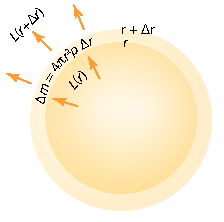
\includegraphics[width=\linewidth]{luminosity-eqn}
\caption[Heat balance in a mass shell]{Heat balance in a shell $\Delta m$.}
\label{f.luminosity}
\end{marginfigure}
\[ 4\pi r^{2}\rho\varepsilon\,\Delta r + L(r) - L(r+\Delta r) = 0. \]
Dividing by $\Delta r$ and taking the limit $\Delta r \to 0$ produces our fourth equation of stellar structure,
\[
\DD{L}{r} = 4\pi r^{2}\rho\varepsilon.
\]
At the center, $L(r)_{r\to0}\to0$, while at the surface $L(r)_{r\to R}\to 4\pi R^{2}\sigmaSB\Teff^{4}$.


